\documentclass[11pt]{article}

\usepackage[T2A]{fontenc}
\usepackage[utf8]{inputenc}
\usepackage[english, russian]{babel}

\usepackage{graphicx}
\graphicspath{ {./liquidcrystalosmosimages/} }

%\usepackage{wrapfig}
%\usepackage[rightcaption]{sidecap}


\begin{document}
    
\title{Жидкокристаллический осмос
или
о возможности нарушения принципа детального равновесия в
жидкокристаллической
дисклинации}
\author{А.Ю. Дроздов}
\date{}

    \maketitle

    А.Ю. Дроздов

    Принцип детального равновесия выводится, например, из следующих общих
представлений: «Вследствие симметрии пространства вероятности состояний
с равными, но противоположно направленными скоростями равны. Поэтому,
если все состояния равны, как это имеет место согласно классической
механике, то для состояния с любой скоростью имеется равновероятное
состояние с противоположной скоростью» {[}А.В.Никулов. «Может ли быть
нарушено второе начало термодинамики без демона Максвелла?»{]}

    Рассматривая данное рассуждение, пренебрежём пока что искривлением
пространства в гравитационном поле Земли. (В скобках заметим, что это
искривление нарушает симметрию пространства, что может в некоторых
случаях приводить к нарушениям принципа детального равновесия. Например:
гравитационно-осмотический кольцар и, предположительно, кольцар
Лазарева, хотя последний требует перепроверки)

    Далее мы покажем, что даже в случае полной симметрии пространства
вероятности состояний с равными, но противоположно направленными
скоростями могут быть неравными, если не равны вероятности
предшествующих состояний, - вследствие детерминизма классической
механики. Иными словами, возьмём некий кадр молекулярного «кино».
Назовём его «центральным» кадром. Зная координаты и скорости всех атомов
можно это «кино» прокрутить как вперёд, так и назад. В первом случае мы
получим состояние, предшествующее центральному кадру, но с
противоположно направленными скоростями, а во втором случае мы получим
состояние предшествующее центральному кадру с «исходно» (или «прямо»)
направленными скоростями.

    Детерминизм классической механики означает уникальность обоих этих
предшествующих (или прокрученных) состояний. То есть получить наш
центральный кадр молекулярного кино можно только лишь из этих
предшествующих состояний, и ни из каких других. Однако эти
предшествующие состояния отличаются друг от друга молекулярной
конфигурацией. И может так случиться, что вероятность этих молекулярных
конфигураций окажутся различными вследствие геометрии опыта.

%\begin{wrapfigure}{l}{0.6\textwidth}
%    \centering
%    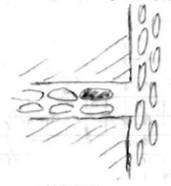
\includegraphics[scale=0.3]{clip_image002.jpg}
%    \caption{кадр назад, состояние 1}
%    \label{fig:frame_back}
%\end{wrapfigure}

\begin{figure}
\centering
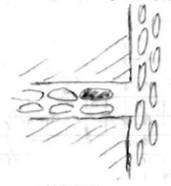
\includegraphics{clip_image002.jpg}
\caption{кадр назад, состояние 1}
\end{figure}

%\begin{wrapfigure}{l}{0.6\textwidth}
%    \centering
%    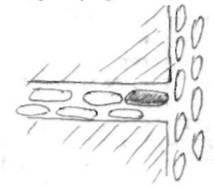
\includegraphics[scale=0.3]{clip_image004.jpg}
%    \caption{центральный кадр, состояние 2}
%    \label{fig:frame_center}
%\end{wrapfigure}

\begin{figure}
\centering
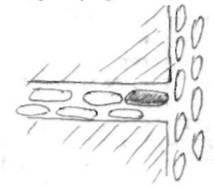
\includegraphics{clip_image004.jpg}
\caption{центральный кадр, состояние 2}
\end{figure}

%\begin{wrapfigure}{l}{0.6\textwidth}
%    \centering
%    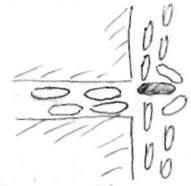
\includegraphics[scale=0.3]{clip_image006.jpg}
%    \caption{кадр вперёд, состояние 3}
%    \label{fig:frame_forword}
%\end{wrapfigure}

\begin{figure}
\centering
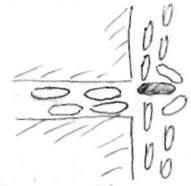
\includegraphics{clip_image006.jpg}
\caption{кадр вперёд, состояние 3}
\end{figure}


    На рисунке изображены одно центральное и два предшествующие состояния,
равновесные вероятности последних могут быть не равны вследствие
ориентационных эффектов в жидком кристалле. Перпендикулярно плоской
поверхности в стекле имеется капилляр. Плоская поверхность благодаря
силам Ван-дер-Ваальса ориентирует молекулы жидкого кристалла вдоль
поверхности. Поверхность капилляра ориентирует молекулы ЖК вдоль
капилляра.

    В устье капилляра есть зона, в которой соседствуют молекулы жидкого
кристалла со взаимно перпендикулярной ориентацией. Эта зона называется
дисклинацией.

Рассмотрим движение молекулы, находящейся в устье капилляра в
непосредственной близости от дисклинации. На рисунке эта молекула
заштрихована. Исследуя принцип детального равновесия, сравним
вероятности состояний, в которых эта молекула имеет скорость v,
направленную вдоль капилляра: в одном случае внутрь капилляра, а в
другом -- наружу.

Если руководствоваться приведенном в начале статьи рассуждением,
основанном на использовании свойств симметрии пространства, то мы придём
к выводу, что состояния с конфигурацией молекул, соответствующей
«центральному» кадру, но с противоположно направленными скоростями имеют
одинаковую энергию (гамильтониан = сумме потенциальной и кинетической
энергий) и на этом основании, казалось бы, эти энергетически равноценные
состояния должны иметь одинаковую вероятность.

Однако вследствие детерминизма классической механики прийти в это
центральное состояние молекулярная система может только из определённых
состояний. В самом деле: обозначим наши состояния как 1, 2 и 3, где 2 --
состояние центрального кадра, 1 -- состояние предшествующего кадра, 3 --
состояние последующего кадра. Дополнительно введём знак + или -- в
качестве индекса для обозначения направления скорости молекул.

Инвариантность уравнений классической механики относительно обращения
времени в совокупности с принципом детерминизма (т.е. в пренебрежении
квантовых эффектов) означает, что:

а) $1+ \rightarrow 2+ \rightarrow 3+$

из состояния 1+ можно прийти только в состояние 2+, а из него -- только
в состояние 3+.

б) $3-- \rightarrow 2-- \rightarrow 1--$

при обращении времени, т.е. при математическом изменении скоростей всех
молекул на противоположные, из состояния 3-- можно прийти только в
состояние 2--, а из него -- только в состояние 1--.

Это значит, что вероятности состояний 1+, 2+ и 3+ равны между собой. А
также то, что вероятности состояний 3-- , 2-- и 1-- равны уже между
собой:

p(1+) = p(2+) = p(3+) = p+

p(3--) = p(2--) = p(1--) = p--

Но это ещё не означает, что вероятности p+ и p--, т.е. вероятности
прямой и обратной ветки, равны между собой. Потому как вероятность
состояния 3-- не обязательно должна быть равна вероятности состояния 1+.
Это может быть хотя бы потому, что ориентация молекул ЖК в состоянии 1
вполне соответствует равновесной ориентации стержнеобразных молекул.
Следовательно, вероятность состояния 1+ относительно высока. С другой
стороны, в состоянии 3 ориентация молекул ЖК (нематика) уже не
соответствует равновесной ориентации молекул. Поэтому вероятность
самопроизвольного возникновения ситуации 3-- из-за флуктуаций нематика в
объёме справа от дисклинации относительно низка. Т.е.:

p(3--) \textless{} p(1+) или p-- \textless{} p+

Читатель может здесь заявить, что всё вышеизложенное абсурд, поскольку
автор предполагает самопроизвольное возникновение неравновесной ситуации
3+ из равновесной 1+.

Совершенно верно! Именно это автор и предполагает, но только, по мнению
автора здесь нет никакого абсурда, а есть проявление диалектической
сущности флуктуаций, как единства и борьбы двух противоположностей. С
одной стороны флуктуации -- явление равновесное, т.к. они существуют в
состоянии термодинамического равновесия. А с другой стороны флуктуации
приводят к локальным микронеравновесностям, примером чего может являться
ситуация 3+.

Всё дело в том, что кинетический механизм образования
микронеравновесности 3+ отличается от механизма образования
микронеравновесности 3--. Для образования состояния 3+ достаточно
наличие достаточно быстро движущейся молекулы слева от дисклинации
направо. Причём это движение должно быть вдоль директора, что
представляется весьма вероятным. Но для образования состояния 3--
необходимо случайно сонаправленное действие многих молекул из области
правее дисклинации. Вероятность чего представляется существенно меньше.

Таким образом мы приходим к выводу, что состояния 2+ и 2--, с одинаковой
конфигурацией молекул, но с противоположно направленными скоростями,
хотя и имеют одинаковые энергии, но они могут иметь различную
вероятность вследствие кинетических причин.

    Теперь рассмотрим броуновское движение молекул в районе дисклинации с
использованием известного уравнения Ланжевена:

\[m\frac{dv}{dt}=F_{Lan}-\gamma \cdot v\]

Проанализируем его составляющую, направленную параллельно капилляру.
Коэффициент вязкости \(\gamma\) справа от дисклинации и слева от
дисклинации неодинаков. Более того, если броуновская частица (молекула
ЖК) пересекает дисклинацию, то весьма вероятно, что коэффициент вязкости
в момент пересечения для частиц пересекающих дисклинацию слева направо
будет ниже, чем таковой для частиц, пересекающих дисклинацию справа
налево. Это так из тех соображений, что стержню, вероятно, легче
проткнуть торцом стопку стержней, чем, если боком напороться на частокол
торцов. Таким образом, для броуновской частицы (молекулы нематика)
блуждающей в районе дисклинации коэффициент вязкости (трения) \(\gamma\)
зависит не только от координаты, но в момент прохождения дисклинации ещё
и от направления скорости. Интегрирование такого уравнения Ланжевена
даст (с учётом того, что средняя сила Ланжевена \(F_{Lan}\) равна нулю)
отличную от нуля среднюю скорость диффузии нематических молекул: слева
направо.

    Теперь разовьём нашу систему капилляров следующим образом. Предположим,
что диаметр капилляра настолько мал, что молекула нематика может
проникнуть в него только вдоль. А поперёк молекула нематика проникнуть в
капилляр не может из-за своей длины. Пусть система таких капилляров даёт
мембрану. Однако поверхности этой мембраны обработаны различным образом.
А именно: поверхность мембраны справа обработана таким образом, что
создаются граничные условия, характерные для планарной (\(\parallel\)
поверхности) ориентации молекул. А поверхность мембраны слева имеет,
скажем, молекулы-ориентанты, создающие граничные условия для
гомеотропной (\(\bot\) поверхности) ориентации молекул.

Известно {[}П. де Жен. Физика жидких кристаллов. М. «Мир», 1977{]}, что
упорядочение длинных осей нематических молекул можно описать функцией
распределения \(f\left(\theta\right)\,sin\,\theta \cdot d\theta\),
дающей вероятность ориентации стержня в телесном угле
\(d\Omega = sin\,\theta \cdot d\theta\) рядом с направлением \(\theta\).
\(f\left(\theta\right) = f\left(\pi - \theta\right)\). Общий вид
\(f\left(\theta\right)\) показан на рисунке.

\begin{figure}
\centering
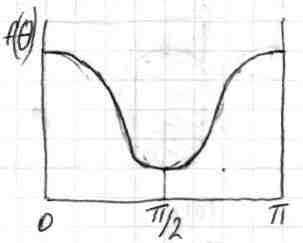
\includegraphics{clip_image024.jpg}
\caption{Общий вид
\(f\left(\theta\right)\)}
\end{figure}

    Сумма по всем телесным углам должна дать полную концентрацию, т.е.:

\(\int f_{\alpha}\left(\theta\right) sin \theta \cdot d\theta = 1\)

Онсангер для \(f\left(\theta\right)\) использовал пробную функцию вида
\(f_{\alpha}\left(\theta\right) = const \cdot ch \left(\alpha \cdot cos \theta \right)\),
где

\(\alpha\) -- вариационный параметр, \(\theta\) -- угол между осью \(a\)
стержня и направлением директора (постоянный множитель определяется
условием нормировки).

$alpha, theta, phi = var("alpha, theta, phi")$
$F_alpha = lambda alpha, theta : cosh (alpha * cos(theta))$

%    \begin{tcolorbox}[breakable, size=fbox, boxrule=1pt, pad at break*=1mm,colback=cellbackground, colframe=cellborder]
%\prompt{In}{incolor}{1}{\boxspacing}
%\begin{Verbatim}[commandchars=\\\{\}]
%\PY{n}{alpha}\PY{p}{,} \PY{n}{theta}\PY{p}{,} \PY{n}{phi} \PY{o}{=} \PY{n}{var}\PY{p}{(}\PY{l+s+s2}{\PYZdq{}}\PY{l+s+s2}{alpha, theta, phi}\PY{l+s+s2}{\PYZdq{}}\PY{p}{)}
%\PY{n}{F\PYZus{}alpha} \PY{o}{=} \PY{k}{lambda} \PY{n}{alpha}\PY{p}{,} \PY{n}{theta} \PY{p}{:} \PY{n}{cosh} \PY{p}{(}\PY{n}{alpha} \PY{o}{*} \PY{n}{cos}\PY{p}{(}\PY{n}{theta}\PY{p}{)}\PY{p}{)}
%\end{Verbatim}
%\end{tcolorbox}

$C = lambda alpha : 1 / numerical_integral(F_alpha(alpha, x), 0, pi) [0]$

%    \begin{tcolorbox}[breakable, size=fbox, boxrule=1pt, pad at break*=1mm,colback=cellbackground, colframe=cellborder]
%\prompt{In}{incolor}{2}{\boxspacing}
%\begin{Verbatim}[commandchars=\\\{\}]
%\PY{n}{C} \PY{o}{=} \PY{k}{lambda} \PY{n}{alpha} \PY{p}{:} \PY{l+m+mi}{1} \PY{o}{/} \PY{n}{numerical\PYZus{}integral}\PY{p}{(}\PY{n}{F\PYZus{}alpha}\PY{p}{(}\PY{n}{alpha}\PY{p}{,} \PY{n}{x}\PY{p}{)}\PY{p}{,} \PY{l+m+mi}{0}\PY{p}{,} \PY{n}{pi}\PY{p}{)} \PY{p}{[}\PY{l+m+mi}{0}\PY{p}{]}
%\end{Verbatim}
%\end{tcolorbox}

$f_alpha = lambda alpha, theta : C(alpha) * F_alpha (alpha, theta)$

%    \begin{tcolorbox}[breakable, size=fbox, boxrule=1pt, pad at break*=1mm,colback=cellbackground, colframe=cellborder]
%\prompt{In}{incolor}{3}{\boxspacing}
%\begin{Verbatim}[commandchars=\\\{\}]
%\PY{n}{f\PYZus{}alpha} \PY{o}{=} \PY{k}{lambda} \PY{n}{alpha}\PY{p}{,} \PY{n}{theta} \PY{p}{:} \PY{n}{C}\PY{p}{(}\PY{n}{alpha}\PY{p}{)} \PY{o}{*} \PY{n}{F\PYZus{}alpha} \PY{p}{(}\PY{n}{alpha}\PY{p}{,} \PY{n}{theta}\PY{p}{)}
%\end{Verbatim}
%\end{tcolorbox}

$plot([f_alpha(0, x), f_alpha(1, x), f_alpha(2, x), f_alpha(3, x), f_alpha(4, x)], x, 0, pi)$

%    \begin{tcolorbox}[breakable, size=fbox, boxrule=1pt, pad at break*=1mm,colback=cellbackground, colframe=cellborder]
%\prompt{In}{incolor}{4}{\boxspacing}
%\begin{Verbatim}[commandchars=\\\{\}]
%\PY{n}{plot}\PY{p}{(}\PY{p}{[}\PY{n}{f\PYZus{}alpha}\PY{p}{(}\PY{l+m+mi}{0}\PY{p}{,} \PY{n}{x}\PY{p}{)}\PY{p}{,} \PY{n}{f\PYZus{}alpha}\PY{p}{(}\PY{l+m+mi}{1}\PY{p}{,} \PY{n}{x}\PY{p}{)}\PY{p}{,} \PY{n}{f\PYZus{}alpha}\PY{p}{(}\PY{l+m+mi}{2}\PY{p}{,} \PY{n}{x}\PY{p}{)}\PY{p}{,} \PY{n}{f\PYZus{}alpha}\PY{p}{(}\PY{l+m+mi}{3}\PY{p}{,} \PY{n}{x}\PY{p}{)}\PY{p}{,} \PY{n}{f\PYZus{}alpha}\PY{p}{(}\PY{l+m+mi}{4}\PY{p}{,} \PY{n}{x}\PY{p}{)}\PY{p}{]}\PY{p}{,} \PY{n}{x}\PY{p}{,} \PY{l+m+mi}{0}\PY{p}{,} \PY{n}{pi}\PY{p}{)}
%\end{Verbatim}
%\end{tcolorbox}
 
            
%\prompt{Out}{outcolor}{4}{}
    
%    \begin{center}
%    \adjustimage{max size={0.9\linewidth}{0.9\paperheight}}{output_17_0.png}
%    \end{center}
%    { \hspace*{\fill} \\}

\begin{figure}
\centering
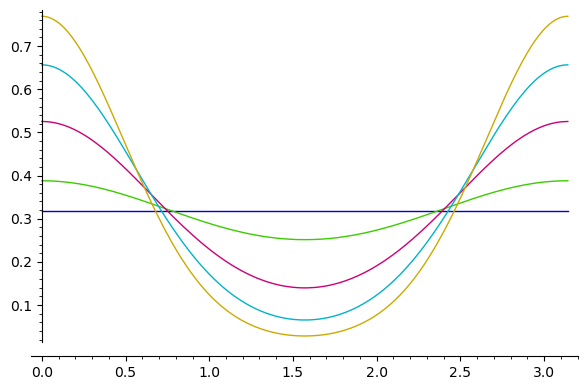
\includegraphics{output_17_0.png}
\caption{output\_17\_0.png}
\end{figure}
    
$tst = lambda alpha : numerical_integral(f_alpha(alpha, theta), 0, pi)[0]$
%    \begin{tcolorbox}[breakable, size=fbox, boxrule=1pt, pad at break*=1mm,colback=cellbackground, colframe=cellborder]
%\prompt{In}{incolor}{5}{\boxspacing}
%\begin{Verbatim}[commandchars=\\\{\}]
%\PY{n}{tst} \PY{o}{=} \PY{k}{lambda} \PY{n}{alpha} \PY{p}{:} \PY{n}{numerical\PYZus{}integral}\PY{p}{(}\PY{n}{f\PYZus{}alpha}\PY{p}{(}\PY{n}{alpha}\PY{p}{,} \PY{n}{theta}\PY{p}{)}\PY{p}{,} \PY{l+m+mi}{0}\PY{p}{,} \PY{n}{pi}\PY{p}{)}\PY{p}{[}\PY{l+m+mi}{0}\PY{p}{]}
%\end{Verbatim}
%\end{tcolorbox}


$tst(0), tst(1), tst(2), tst(3)$
%    \begin{tcolorbox}[breakable, size=fbox, boxrule=1pt, pad at break*=1mm,colback=cellbackground, colframe=cellborder]
%\prompt{In}{incolor}{6}{\boxspacing}
%\begin{Verbatim}[commandchars=\\\{\}]
%\PY{n}{tst}\PY{p}{(}\PY{l+m+mi}{0}\PY{p}{)}\PY{p}{,} \PY{n}{tst}\PY{p}{(}\PY{l+m+mi}{1}\PY{p}{)}\PY{p}{,} \PY{n}{tst}\PY{p}{(}\PY{l+m+mi}{2}\PY{p}{)}\PY{p}{,} \PY{n}{tst}\PY{p}{(}\PY{l+m+mi}{3}\PY{p}{)}
%\end{Verbatim}
%\end{tcolorbox}

%            \begin{tcolorbox}[breakable, size=fbox, boxrule=.5pt, pad at break*=1mm, opacityfill=0]
%\prompt{Out}{outcolor}{6}{\boxspacing}
%\begin{Verbatim}[commandchars=\\\{\}]
(1.0, 0.9999999999999999, 0.9999999999999997, 0.9999999999999997)
%\end{Verbatim}
%\end{tcolorbox}
        
    Параметр порядка:

\begin{equation}
S=\frac{1}{2}\left<\left(3\,cos^{2} \theta - 1 \right)\right> =
\int f\left(\theta\right)\frac{1}{2}\left(3\,cos^2\theta - 1\right)\,d\Omega =
\int f_{\alpha}\frac{1}{2}\left(3\,cos^2\theta - 1\right)\,sin\,\theta\,d\theta \approx 1-\frac{3}{\alpha}
\end{equation}

$S = lambda alpha : integral(f_alpha(alpha, theta)*1/2*(3*cos(theta)^2-1)*sin(theta), theta, 0, pi)$

%    \begin{tcolorbox}[breakable, size=fbox, boxrule=1pt, pad at break*=1mm,colback=cellbackground, colframe=cellborder]
%\prompt{In}{incolor}{7}{\boxspacing}
%\begin{Verbatim}[commandchars=\\\{\}]
%\PY{n}{S} \PY{o}{=} \PY{k}{lambda} \PY{n}{alpha} \PY{p}{:} \PY{n}{integral}\PY{p}{(}\PY{n}{f\PYZus{}alpha}\PY{p}{(}\PY{n}{alpha}\PY{p}{,} \PY{n}{theta}\PY{p}{)}\PY{o}{*}\PY{l+m+mi}{1}\PY{o}{/}\PY{l+m+mi}{2}\PY{o}{*}\PY{p}{(}\PY{l+m+mi}{3}\PY{o}{*}\PY{n}{cos}\PY{p}{(}\PY{n}{theta}\PY{p}{)}\PY{o}{\PYZca{}}\PY{l+m+mi}{2}\PY{o}{\PYZhy{}}\PY{l+m+mi}{1}\PY{p}{)}\PY{o}{*}\PY{n}{sin}\PY{p}{(}\PY{n}{theta}\PY{p}{)}\PY{p}{,} \PY{n}{theta}\PY{p}{,} \PY{l+m+mi}{0}\PY{p}{,} \PY{n}{pi}\PY{p}{)} 
%\end{Verbatim}
%\end{tcolorbox}


$plot(S(x), x, 0, 4)$
%    \begin{tcolorbox}[breakable, size=fbox, boxrule=1pt, pad at break*=1mm,colback=cellbackground, colframe=cellborder]
%\prompt{In}{incolor}{8}{\boxspacing}
%\begin{Verbatim}[commandchars=\\\{\}]
%\PY{n}{plot}\PY{p}{(}\PY{n}{S}\PY{p}{(}\PY{n}{x}\PY{p}{)}\PY{p}{,} \PY{n}{x}\PY{p}{,} \PY{l+m+mi}{0}\PY{p}{,} \PY{l+m+mi}{4}\PY{p}{)}
%\end{Verbatim}
%\end{tcolorbox}
 
            
%\prompt{Out}{outcolor}{8}{}
    
%    \begin{center}
%    \adjustimage{max size={0.9\linewidth}{0.9\paperheight}}{output_22_0.png}
%    \end{center}
%    { \hspace*{\fill} \\}

\begin{figure}
\centering
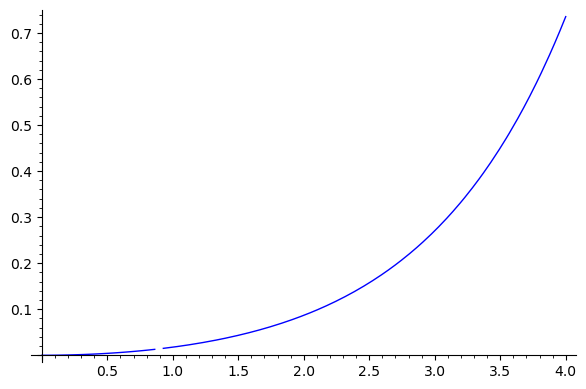
\includegraphics{output_22_0.png}
\caption{output\_22\_0.png}
\end{figure}

    \begin{figure}
\centering
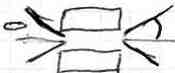
\includegraphics{clip_image032.jpg}
\caption{clip\_image032.gif}
\end{figure}

Предположим, что шанс проникнуть внутрь капилляра в результате диффузии
имеют молекулы ориентированные внутри телесного угла
\(\Omega_{\,0} = \int \limits_{0}^{2 \pi}d\varphi'\int\limits_{0}^{\theta_{0}}sin\,\theta'\,d\theta'\).

    Таким образом, концентрация молекул, которые имеют шанс проникнуть в
мембрану слева (поверхность мембраны слева имеет, как мы условились,
молекулы-ориентанты, создающие граничные условия для гомеотропной
(\(\bot\) поверхности) ориентации молекул):


\[c_{\bot}=c\cdot\frac{\int \limits{\Omega_{\,0}}^{}f_{\alpha}\,d\Omega}{2\pi}\]

\[c_{\bot}=c\,\int \limits{0}^{\theta_{0}}f_{\alpha}\left(\theta\right)\,sin\,\theta\,d\theta\]

данная формула выводится очень просто потому что для гомеотропной
(\(\bot\) поверхности) ориентации молекул сферическая координата
\(\theta'\) телесного угла \(\Omega_{\,0}\) и угол отклонения ориентации
стержня \(\theta\) от направления директора жидкого кристалла совпадают.

Однако это не так для для планарной (\(\parallel\) поверхности)
ориентации молекул. Для нее сферическая система координат
\(\theta', \varphi'\) в которой строится телесный угол \(\Omega_{\,0}\)
вероятности проникновения в капилляр и сферическая система координат
\(\theta, \varphi\) отклонения молекул стержней построенная относительно
направление директора жидкого кристалла отклонены на 90 градусов.

\[c_{\parallel}=c\cdot\frac{\int \limits_{0}^{2 \pi}\int\limits_{0}^{\theta_{0}}f_{\alpha}\left(\theta\right)sin\,\theta'\,d\theta'd\varphi'}{2\pi}\]

Для взятия этого итеграла переходим из сферических координат в декартовы

\(x'= r\,sin \theta'\,cos \varphi'\)

\(y'= r\,sin \theta'\,sin \varphi'\)

\(z'= r\,cos \theta'\),

делаем поворот декартовых осей

\(z = y'\)

\(x = x'\)

\(y = -z'\)

и из них переходим в новые сферические

\(\theta = arccos\frac{z}{\sqrt{x^2+y^2+z^2}}\)

\(\theta = arccos\frac{y'}{\sqrt{x'^2+y'^2+z'^2}}\)

\(\theta = arccos\left(sin \theta'\,sin \varphi'\right)\)

концентрация молекул, которые имеют шанс проникнуть в мембрану для
молекул справа (поверхность мембраны справа обработана таким образом,
что создаются граничные условия, характерные для планарной
(\(\parallel\) поверхности) ориентации молекул):

\[c_{\parallel}=c\cdot\frac{\int \limits_{0}^{2 \pi}\int\limits_{0}^{\theta_{0}}f_{\alpha}\left(arccos\left(sin \theta'\,sin \varphi'\right)\right)sin\,\theta'\,d\theta'd\varphi'}{2\pi}\]

    Разность этих концентраций \(c_{\bot}-c_{\parallel}\) графически можно
определить, как отношение площади заштрихованной области к общей площади
под графиком, умноженное на общую концентрацию \(c\)

\[\Delta c = c_{\bot}-c_{\parallel} = \beta \cdot c\]

Коэффициент \(\beta\) можно оценить численно исходя из вышеприведенного
приближения Онсангера для \(f_{\alpha}\).

    \[c_{\bot}=c\,\int \limits{0}^{\theta_{0}}f_{\alpha}\left(\theta\right)\,sin\,\theta\,d\theta\]

$theta_0 = var("theta_0")$

$c_gomeotrop = lambda theta_0, alpha : numerical_integral(f_alpha(alpha, theta)*sin(theta), 0, theta_0)[0]$

%    \begin{tcolorbox}[breakable, size=fbox, boxrule=1pt, pad at break*=1mm,colback=cellbackground, colframe=cellborder]
%\prompt{In}{incolor}{9}{\boxspacing}
%\begin{Verbatim}[commandchars=\\\{\}]
%\PY{n}{theta\PYZus{}0} \PY{o}{=} \PY{n}{var}\PY{p}{(}\PY{l+s+s2}{\PYZdq{}}\PY{l+s+s2}{theta\PYZus{}0}\PY{l+s+s2}{\PYZdq{}}\PY{p}{)}
%\PY{n}{c\PYZus{}gomeotrop} \PY{o}{=} \PY{k}{lambda} \PY{n}{theta\PYZus{}0}\PY{p}{,} \PY{n}{alpha} \PY{p}{:} \PY{n}{numerical\PYZus{}integral}\PY{p}{(}\PY{n}{f\PYZus{}alpha}\PY{p}{(}\PY{n}{alpha}\PY{p}{,} \PY{n}{theta}\PY{p}{)}\PY{o}{*}\PY{n}{sin}\PY{p}{(}\PY{n}{theta}\PY{p}{)}\PY{p}{,} \PY{l+m+mi}{0}\PY{p}{,} \PY{n}{theta\PYZus{}0}\PY{p}{)}\PY{p}{[}\PY{l+m+mi}{0}\PY{p}{]}
%\end{Verbatim}
%\end{tcolorbox}

$rotated_theta = lambda theta, phi : acos(sin(theta)*sin(phi))$

%    \begin{tcolorbox}[breakable, size=fbox, boxrule=1pt, pad at break*=1mm,colback=cellbackground, colframe=cellborder]
%\prompt{In}{incolor}{10}{\boxspacing}
%\begin{Verbatim}[commandchars=\\\{\}]
%\PY{n}{rotated\PYZus{}theta} \PY{o}{=} \PY{k}{lambda} \PY{n}{theta}\PY{p}{,} \PY{n}{phi} \PY{p}{:} \PY{n}{acos}\PY{p}{(}\PY{n}{sin}\PY{p}{(}\PY{n}{theta}\PY{p}{)}\PY{o}{*}\PY{n}{sin}\PY{p}{(}\PY{n}{phi}\PY{p}{)}\PY{p}{)}
%\end{Verbatim}
%\end{tcolorbox}

$rotated_theta (pi/6, 2*pi)$

%    \begin{tcolorbox}[breakable, size=fbox, boxrule=1pt, pad at break*=1mm,colback=cellbackground, colframe=cellborder]
%\prompt{In}{incolor}{11}{\boxspacing}
%\begin{Verbatim}[commandchars=\\\{\}]
%\PY{n}{rotated\PYZus{}theta} \PY{p}{(}\PY{n}{pi}\PY{o}{/}\PY{l+m+mi}{6}\PY{p}{,} \PY{l+m+mi}{2}\PY{o}{*}\PY{n}{pi}\PY{p}{)}
%\end{Verbatim}
%\end{tcolorbox}

%            \begin{tcolorbox}[breakable, size=fbox, boxrule=.5pt, pad at break*=1mm, opacityfill=0]
%\prompt{Out}{outcolor}{11}{\boxspacing}
%\begin{Verbatim}[commandchars=\\\{\}]
$1/2*pi$
%\end{Verbatim}
%\end{tcolorbox}
        
    \[c_{\parallel}=c\cdot\frac{\int \limits_{0}^{2 \pi}\int\limits_{0}^{\theta_{0}}f_{\alpha}\left(\theta\right)sin\,\theta'\,d\theta'd\varphi'}{2\pi}\]


$$c_planar = lambda theta_0, alpha : 1/(2*pi) * \
    numerical_integral(\
        lambda theta : numerical_integral( \
            lambda phi : f_alpha(alpha, rotated_theta(theta, phi)) * sin(theta)\
                           , 0, 2*pi)[0] \
                      , 0, theta_0)[0]$$
%    \begin{tcolorbox}[breakable, size=fbox, boxrule=1pt, pad at break*=1mm,colback=cellbackground, colframe=cellborder]
%\prompt{In}{incolor}{12}{\boxspacing}
%\begin{Verbatim}[commandchars=\\\{\}]
%\PY{n}{c\PYZus{}planar} \PY{o}{=} \PY{k}{lambda} \PY{n}{theta\PYZus{}0}\PY{p}{,} \PY{n}{alpha} \PY{p}{:} \PY{l+m+mi}{1}\PY{o}{/}\PY{p}{(}\PY{l+m+mi}{2}\PY{o}{*}\PY{n}{pi}\PY{p}{)} \PY{o}{*} \PYZbs{}
%    \PY{n}{numerical\PYZus{}integral}\PY{p}{(}\PYZbs{}
%        \PY{k}{lambda} \PY{n}{theta} \PY{p}{:} \PY{n}{numerical\PYZus{}integral}\PY{p}{(} \PYZbs{}
%            \PY{k}{lambda} \PY{n}{phi} \PY{p}{:} \PY{n}{f\PYZus{}alpha}\PY{p}{(}\PY{n}{alpha}\PY{p}{,} \PY{n}{rotated\PYZus{}theta}\PY{p}{(}\PY{n}{theta}\PY{p}{,} \PY{n}{phi}\PY{p}{)}\PY{p}{)} \PY{o}{*} \PY{n}{sin}\PY{p}{(}\PY{n}{theta}\PY{p}{)}\PYZbs{}
%                           \PY{p}{,} \PY{l+m+mi}{0}\PY{p}{,} \PY{l+m+mi}{2}\PY{o}{*}\PY{n}{pi}\PY{p}{)}\PY{p}{[}\PY{l+m+mi}{0}\PY{p}{]} \PYZbs{}
%                      \PY{p}{,} \PY{l+m+mi}{0}\PY{p}{,} \PY{n}{theta\PYZus{}0}\PY{p}{)}\PY{p}{[}\PY{l+m+mi}{0}\PY{p}{]}
%\end{Verbatim}
%\end{tcolorbox}

$$beta = lambda theta_0, alpha : c_gomeotrop(theta_0, alpha) - c_planar(theta_0, alpha)$$

%    \begin{tcolorbox}[breakable, size=fbox, boxrule=1pt, pad at break*=1mm,colback=cellbackground, colframe=cellborder]
%\prompt{In}{incolor}{13}{\boxspacing}
%\begin{Verbatim}[commandchars=\\\{\}]
%\PY{n}{beta} \PY{o}{=} \PY{k}{lambda} \PY{n}{theta\PYZus{}0}\PY{p}{,} \PY{n}{alpha} \PY{p}{:} \PY{n}{c\PYZus{}gomeotrop}\PY{p}{(}\PY{n}{theta\PYZus{}0}\PY{p}{,} \PY{n}{alpha}\PY{p}{)} \PY{o}{\PYZhy{}} \PY{n}{c\PYZus{}planar}\PY{p}{(}\PY{n}{theta\PYZus{}0}\PY{p}{,} \PY{n}{alpha}\PY{p}{)}
%\end{Verbatim}
%\end{tcolorbox}

$c_gomeotrop(pi/4, 1)$

%    \begin{tcolorbox}[breakable, size=fbox, boxrule=1pt, pad at break*=1mm,colback=cellbackground, colframe=cellborder]
%\prompt{In}{incolor}{14}{\boxspacing}
%\begin{Verbatim}[commandchars=\\\{\}]
%\PY{n}{c\PYZus{}gomeotrop}\PY{p}{(}\PY{n}{pi}\PY{o}{/}\PY{l+m+mi}{4}\PY{p}{,} \PY{l+m+mi}{1}\PY{p}{)}
%\end{Verbatim}
%\end{tcolorbox}

%            \begin{tcolorbox}[breakable, size=fbox, boxrule=.5pt, pad at break*=1mm, opacityfill=0]
%\prompt{Out}{outcolor}{14}{\boxspacing}
%\begin{Verbatim}[commandchars=\\\{\}]
0.1024969991717229
%\end{Verbatim}
%\end{tcolorbox}
        

$c_planar(pi/4, 1).n()$
%    \begin{tcolorbox}[breakable, size=fbox, boxrule=1pt, pad at break*=1mm,colback=cellbackground, colframe=cellborder]
%\prompt{In}{incolor}{15}{\boxspacing}
%\begin{Verbatim}[commandchars=\\\{\}]
%\PY{n}{c\PYZus{}planar}\PY{p}{(}\PY{n}{pi}\PY{o}{/}\PY{l+m+mi}{4}\PY{p}{,} \PY{l+m+mi}{1}\PY{p}{)}\PY{o}{.}\PY{n}{n}\PY{p}{(}\PY{p}{)}
%\end{Verbatim}
%\end{tcolorbox}

%            \begin{tcolorbox}[breakable, size=fbox, boxrule=.5pt, pad at break*=1mm, opacityfill=0]
%\prompt{Out}{outcolor}{15}{\boxspacing}
%\begin{Verbatim}[commandchars=\\\{\}]
0.0786093035482243
%\end{Verbatim}
%\end{tcolorbox}
        
    \(\beta\) сильно зависит от \(\theta_{0}\) (а последний, судя по всему,
определяется диаметром капилляра). Кроме того, \(\beta\) пропорционален
параметру порядка S.


%plot_data_beta = []
%theta_0_i = 3/4*pi/2
%for alpha_i in (0, 1, 2, 3, 4.0, 4.5, 5.0, 5.5):
%    b = beta(theta_0_i, alpha_i).n()
%    print(theta_0_i, alpha_i, b)
%    plot_data_beta += [(alpha_i, b)]
%list_plot(plot_data_beta).show(title = "\beta on \alpha with \theta_0 = " + str(theta_0_i))

%    \begin{tcolorbox}[breakable, size=fbox, boxrule=1pt, pad at break*=1mm,colback=cellbackground, colframe=cellborder]
%\prompt{In}{incolor}{16}{\boxspacing}
%\begin{Verbatim}[commandchars=\\\{\}]
%\PY{n}{plot\PYZus{}data\PYZus{}beta} \PY{o}{=} \PY{p}{[}\PY{p}{]}

%\PY{n}{theta\PYZus{}0\PYZus{}i} \PY{o}{=} \PY{l+m+mi}{3}\PY{o}{/}\PY{l+m+mi}{4}\PY{o}{*}\PY{n}{pi}\PY{o}{/}\PY{l+m+mi}{2}
%\PY{k}{for} \PY{n}{alpha\PYZus{}i} \PY{o+ow}{in} \PY{p}{(}\PY{l+m+mi}{0}\PY{p}{,} \PY{l+m+mi}{1}\PY{p}{,} \PY{l+m+mi}{2}\PY{p}{,} \PY{l+m+mi}{3}\PY{p}{,} \PY{l+m+mf}{4.0}\PY{p}{,} \PY{l+m+mf}{4.5}\PY{p}{,} \PY{l+m+mf}{5.0}\PY{p}{,} \PY{l+m+mf}{5.5}\PY{p}{)}\PY{p}{:}
%    \PY{n}{b} \PY{o}{=} \PY{n}{beta}\PY{p}{(}\PY{n}{theta\PYZus{}0\PYZus{}i}\PY{p}{,} \PY{n}{alpha\PYZus{}i}\PY{p}{)}\PY{o}{.}\PY{n}{n}\PY{p}{(}\PY{p}{)}
%    \PY{n+nb}{print}\PY{p}{(}\PY{n}{theta\PYZus{}0\PYZus{}i}\PY{p}{,} \PY{n}{alpha\PYZus{}i}\PY{p}{,} \PY{n}{b}\PY{p}{)}
%    \PY{n}{plot\PYZus{}data\PYZus{}beta} \PY{o}{+}\PY{o}{=} \PY{p}{[}\PY{p}{(}\PY{n}{alpha\PYZus{}i}\PY{p}{,} \PY{n}{b}\PY{p}{)}\PY{p}{]}
%\PY{n}{list\PYZus{}plot}\PY{p}{(}\PY{n}{plot\PYZus{}data\PYZus{}beta}\PY{p}{)}\PY{o}{.}\PY{n}{show}\PY{p}{(}\PY{n}{title} \PY{o}{=} \PY{l+s+s2}{\PYZdq{}}\PY{l+s+s2}{\PYZdl{}}\PY{l+s+se}{\PYZbs{}\PYZbs{}}\PY{l+s+s2}{beta\PYZdl{} on \PYZdl{}}\PY{l+s+se}{\PYZbs{}\PYZbs{}}\PY{l+s+s2}{alpha\PYZdl{} with \PYZdl{}}\PY{l+s+se}{\PYZbs{}\PYZbs{}}\PY{l+s+s2}{theta\PYZus{}0 = \PYZdl{}}\PY{l+s+s2}{\PYZdq{}} \PY{o}{+} \PY{n+nb}{str}\PY{p}{(}\PY{n}{theta\PYZus{}0\PYZus{}i}\PY{p}{)}\PY{p}{)}
%\end{Verbatim}
%\end{tcolorbox}

%    \begin{Verbatim}[commandchars=\\\{\}]
3/8*pi 0 0.000000000000000
3/8*pi 1 0.0219131769483767
3/8*pi 2 0.0589328777829388
3/8*pi 3 0.0840390756546801
3/8*pi 4.00000000000000 0.0966065629923601
3/8*pi 4.50000000000000 0.0998441868232591
3/8*pi 5.00000000000000 0.101782406973619
3/8*pi 5.50000000000000 0.102804518664355
%    \end{Verbatim}
    
\begin{figure}
\centering
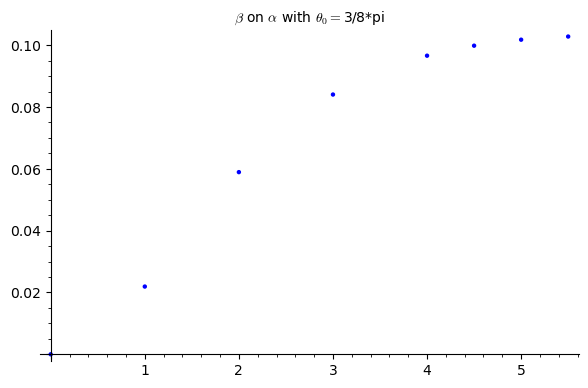
\includegraphics{output_36_1.png}
\caption{output\_36\_1.png}
\end{figure}


%$$plot_data_beta = []
%theta_0_i = pi/4
%for alpha_i in (0, 1, 2, 3, 4.0, 4.5, 5.0, 5.5):
%    b = beta(theta_0_i, alpha_i).n()
%    print(theta_0_i, alpha_i, b)
%    plot_data_beta += [(alpha_i, b)]
%list_plot(plot_data_beta).show(title = "$\\beta$ on $\\alpha$ with $\\theta_0 = $" + str(theta_0_i))$$

%    \begin{tcolorbox}[breakable, size=fbox, boxrule=1pt, pad at break*=1mm,colback=cellbackground, colframe=cellborder]
%\prompt{In}{incolor}{17}{\boxspacing}
%\begin{Verbatim}[commandchars=\\\{\}]
%\PY{n}{plot\PYZus{}data\PYZus{}beta} \PY{o}{=} \PY{p}{[}\PY{p}{]}

%\PY{n}{theta\PYZus{}0\PYZus{}i} \PY{o}{=} \PY{n}{pi}\PY{o}{/}\PY{l+m+mi}{4}
%\PY{k}{for} \PY{n}{alpha\PYZus{}i} \PY{o+ow}{in} \PY{p}{(}\PY{l+m+mi}{0}\PY{p}{,} \PY{l+m+mi}{1}\PY{p}{,} \PY{l+m+mi}{2}\PY{p}{,} \PY{l+m+mi}{3}\PY{p}{,} \PY{l+m+mf}{4.0}\PY{p}{,} \PY{l+m+mf}{4.5}\PY{p}{,} \PY{l+m+mf}{5.0}\PY{p}{,} \PY{l+m+mf}{5.5}\PY{p}{)}\PY{p}{:}
%    \PY{n}{b} \PY{o}{=} \PY{n}{beta}\PY{p}{(}\PY{n}{theta\PYZus{}0\PYZus{}i}\PY{p}{,} \PY{n}{alpha\PYZus{}i}\PY{p}{)}\PY{o}{.}\PY{n}{n}\PY{p}{(}\PY{p}{)}
%    \PY{n+nb}{print}\PY{p}{(}\PY{n}{theta\PYZus{}0\PYZus{}i}\PY{p}{,} \PY{n}{alpha\PYZus{}i}\PY{p}{,} \PY{n}{b}\PY{p}{)}
%    \PY{n}{plot\PYZus{}data\PYZus{}beta} \PY{o}{+}\PY{o}{=} \PY{p}{[}\PY{p}{(}\PY{n}{alpha\PYZus{}i}\PY{p}{,} \PY{n}{b}\PY{p}{)}\PY{p}{]}
%\PY{n}{list\PYZus{}plot}\PY{p}{(}\PY{n}{plot\PYZus{}data\PYZus{}beta}\PY{p}{)}\PY{o}{.}\PY{n}{show}\PY{p}{(}\PY{n}{title} \PY{o}{=} \PY{l+s+s2}{\PYZdq{}}\PY{l+s+s2}{\PYZdl{}}\PY{l+s+se}{\PYZbs{}\PYZbs{}}\PY{l+s+s2}{beta\PYZdl{} on \PYZdl{}}\PY{l+s+se}{\PYZbs{}\PYZbs{}}\PY{l+s+s2}{alpha\PYZdl{} with \PYZdl{}}\PY{l+s+se}{\PYZbs{}\PYZbs{}}\PY{l+s+s2}{theta\PYZus{}0 = \PYZdl{}}\PY{l+s+s2}{\PYZdq{}} \PY{o}{+} \PY{n+nb}{str}\PY{p}{(}\PY{n}{theta\PYZus{}0\PYZus{}i}\PY{p}{)}\PY{p}{)}
%\end{Verbatim}
%\end{tcolorbox}

%    \begin{Verbatim}[commandchars=\\\{\}]
1/4*pi 0 -2.77555756156289e-17
1/4*pi 1 0.0238876956234986
1/4*pi 2 0.0654413340746269
1/4*pi 3 0.0955303686898020
1/4*pi 4.00000000000000 0.112267703109153
1/4*pi 4.50000000000000 0.117107187799921
1/4*pi 5.00000000000000 0.120302057514500
1/4*pi 5.50000000000000 0.122247865168600
%    \end{Verbatim}

%    \begin{center}
%    \adjustimage{max size={0.9\linewidth}{0.9\paperheight}}{output_37_1.png}
%    \end{center}
%    { \hspace*{\fill} \\}

\begin{figure}
\centering
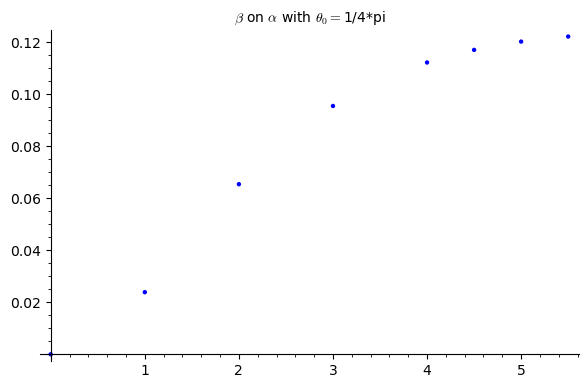
\includegraphics{output_37_1.png}
\caption{output\_37\_1.png}
\end{figure}


%$$plot_data_beta = []
%theta_0_i = pi/6
%for alpha_i in (0, 1, 2, 3, 4.0, 4.5, 5.0, 5.5):
%    b = beta(theta_0_i, alpha_i).n()
%    print(theta_0_i, alpha_i, b)
%    plot_data_beta += [(alpha_i, b)]
%list_plot(plot_data_beta).show(title = "$\\beta$ on $\\alpha$ with $\\theta_0 = $" + str(theta_0_i))$$
    
%    \begin{tcolorbox}[breakable, size=fbox, boxrule=1pt, pad at break*=1mm,colback=cellbackground, colframe=cellborder]
%\prompt{In}{incolor}{18}{\boxspacing}
%\begin{Verbatim}[commandchars=\\\{\}]
%\PY{n}{plot\PYZus{}data\PYZus{}beta} \PY{o}{=} \PY{p}{[}\PY{p}{]}

%\PY{n}{theta\PYZus{}0\PYZus{}i} \PY{o}{=} \PY{n}{pi}\PY{o}{/}\PY{l+m+mi}{6}
%\PY{k}{for} \PY{n}{alpha\PYZus{}i} \PY{o+ow}{in} \PY{p}{(}\PY{l+m+mi}{0}\PY{p}{,} \PY{l+m+mi}{1}\PY{p}{,} \PY{l+m+mi}{2}\PY{p}{,} \PY{l+m+mi}{3}\PY{p}{,} \PY{l+m+mf}{4.0}\PY{p}{,} \PY{l+m+mf}{4.5}\PY{p}{,} \PY{l+m+mf}{5.0}\PY{p}{,} \PY{l+m+mf}{5.5}\PY{p}{)}\PY{p}{:}
%    \PY{n}{b} \PY{o}{=} \PY{n}{beta}\PY{p}{(}\PY{n}{theta\PYZus{}0\PYZus{}i}\PY{p}{,} \PY{n}{alpha\PYZus{}i}\PY{p}{)}\PY{o}{.}\PY{n}{n}\PY{p}{(}\PY{p}{)}
%    \PY{n+nb}{print}\PY{p}{(}\PY{n}{theta\PYZus{}0\PYZus{}i}\PY{p}{,} \PY{n}{alpha\PYZus{}i}\PY{p}{,} \PY{n}{b}\PY{p}{)}
%    \PY{n}{plot\PYZus{}data\PYZus{}beta} \PY{o}{+}\PY{o}{=} \PY{p}{[}\PY{p}{(}\PY{n}{alpha\PYZus{}i}\PY{p}{,} \PY{n}{b}\PY{p}{)}\PY{p}{]}
%\PY{n}{list\PYZus{}plot}\PY{p}{(}\PY{n}{plot\PYZus{}data\PYZus{}beta}\PY{p}{)}\PY{o}{.}\PY{n}{show}\PY{p}{(}\PY{n}{title} \PY{o}{=} \PY{l+s+s2}{\PYZdq{}}\PY{l+s+s2}{\PYZdl{}}\PY{l+s+se}{\PYZbs{}\PYZbs{}}\PY{l+s+s2}{beta\PYZdl{} on \PYZdl{}}\PY{l+s+se}{\PYZbs{}\PYZbs{}}\PY{l+s+s2}{alpha\PYZdl{} with \PYZdl{}}\PY{l+s+se}{\PYZbs{}\PYZbs{}}\PY{l+s+s2}{theta\PYZus{}0 = \PYZdl{}}\PY{l+s+s2}{\PYZdq{}} \PY{o}{+} \PY{n+nb}{str}\PY{p}{(}\PY{n}{theta\PYZus{}0\PYZus{}i}\PY{p}{)}\PY{p}{)}
%\end{Verbatim}
%\end{tcolorbox}

%    \begin{Verbatim}[commandchars=\\\{\}]
1/6*pi 0 -2.08166817117217e-17
1/6*pi 1 0.0147035756341011
1/6*pi 2 0.0408769322394912
1/6*pi 3 0.0610204690320465
1/6*pi 4.00000000000000 0.0737273449761888
1/6*pi 4.50000000000000 0.0780819667950208
1/6*pi 5.00000000000000 0.0814843952803334
1/6*pi 5.50000000000000 0.0841445593843594
%    \end{Verbatim}

    
\begin{figure}
\centering
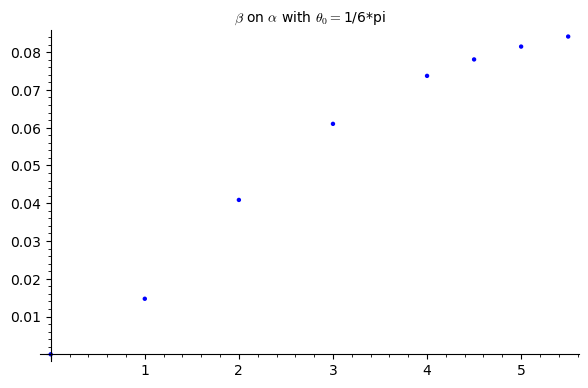
\includegraphics{output_38_1.png}
\caption{"$\beta on \alpha with \theta_0 =  \pi/6$" }
\end{figure}

%
%plot_data_beta = []
%alpha_i = 4
%for i in range(0,64+1):
%    theta_0_i = i * pi/128
%    b = beta(theta_0_i, alpha_i).n()
%    print(theta_0_i, alpha_i, b)
%    plot_data_beta += [(theta_0_i/pi*2, b)]
%list_plot(plot_data_beta).show(title = "$\\beta$ on $\\theta_0$ with $\\alpha = $" + str(alpha_i))


%    \begin{tcolorbox}[breakable, size=fbox, boxrule=1pt, pad at break*=1mm,colback=cellbackground, colframe=cellborder]
%\prompt{In}{incolor}{19}{\boxspacing}
%\begin{Verbatim}[commandchars=\\\{\}]
%\PY{n}{plot\PYZus{}data\PYZus{}beta} \PY{o}{=} \PY{p}{[}\PY{p}{]}

%\PY{n}{alpha\PYZus{}i} \PY{o}{=} \PY{l+m+mi}{4}
%\PY{k}{for} \PY{n}{i} \PY{o+ow}{in} \PY{n+nb}{range}\PY{p}{(}\PY{l+m+mi}{0}\PY{p}{,}\PY{l+m+mi}{64}\PY{o}{+}\PY{l+m+mi}{1}\PY{p}{)}\PY{p}{:}
%    \PY{n}{theta\PYZus{}0\PYZus{}i} \PY{o}{=} \PY{n}{i} \PY{o}{*} \PY{n}{pi}\PY{o}{/}\PY{l+m+mi}{128}
%    \PY{n}{b} \PY{o}{=} \PY{n}{beta}\PY{p}{(}\PY{n}{theta\PYZus{}0\PYZus{}i}\PY{p}{,} \PY{n}{alpha\PYZus{}i}\PY{p}{)}\PY{o}{.}\PY{n}{n}\PY{p}{(}\PY{p}{)}
%    \PY{n+nb}{print}\PY{p}{(}\PY{n}{theta\PYZus{}0\PYZus{}i}\PY{p}{,} \PY{n}{alpha\PYZus{}i}\PY{p}{,} \PY{n}{b}\PY{p}{)}
%    \PY{n}{plot\PYZus{}data\PYZus{}beta} \PY{o}{+}\PY{o}{=} \PY{p}{[}\PY{p}{(}\PY{n}{theta\PYZus{}0\PYZus{}i}\PY{o}{/}\PY{n}{pi}\PY{o}{*}\PY{l+m+mi}{2}\PY{p}{,} \PY{n}{b}\PY{p}{)}\PY{p}{]}
%\PY{n}{list\PYZus{}plot}\PY{p}{(}\PY{n}{plot\PYZus{}data\PYZus{}beta}\PY{p}{)}\PY{o}{.}\PY{n}{show}\PY{p}{(}\PY{n}{title} \PY{o}{=} \PY{l+s+s2}{\PYZdq{}}\PY{l+s+s2}{\PYZdl{}}\PY{l+s+se}{\PYZbs{}\PYZbs{}}\PY{l+s+s2}{beta\PYZdl{} on \PYZdl{}}\PY{l+s+se}{\PYZbs{}\PYZbs{}}\PY{l+s+s2}{theta\PYZus{}0\PYZdl{} with \PYZdl{}}\PY{l+s+se}{\PYZbs{}\PYZbs{}}\PY{l+s+s2}{alpha = \PYZdl{}}\PY{l+s+s2}{\PYZdq{}} \PY{o}{+} \PY{n+nb}{str}\PY{p}{(}\PY{n}{alpha\PYZus{}i}\PY{p}{)}\PY{p}{)}
%\end{Verbatim}
%\end{tcolorbox}

%    \begin{Verbatim}[commandchars=\\\{\}]
0 4 0.000000000000000
1/128*pi 4 0.000223010988522073
1/64*pi 4 0.000890117518740633
3/128*pi 4 0.00199556471439369
1/32*pi 4 0.00352984204003176
5/128*pi 4 0.00547980292641991
3/64*pi 4 0.00782882877390517
7/128*pi 4 0.0105570339809177
1/16*pi 4 0.0136415078525885
9/128*pi 4 0.0170565885685088
5/64*pi 4 0.0207741638461873
11/128*pi 4 0.0247639925404763
3/32*pi 4 0.0289940411769287
13/128*pi 4 0.0334308293314283
7/64*pi 4 0.0380397778372340
15/128*pi 4 0.0427855540167144
1/8*pi 4 0.0476324084871105
17/128*pi 4 0.0525444985624011
9/64*pi 4 0.0574861938483839
19/128*pi 4 0.0624223602846818
5/32*pi 4 0.0673186196032069
21/128*pi 4 0.0721415819245910
11/64*pi 4 0.0768590499792096
23/128*pi 4 0.0814401941954379
3/16*pi 4 0.0858556986239478
25/128*pi 4 0.0900778783444535
13/64*pi 4 0.0940807696141474
27/128*pi 4 0.0978401945517801
7/32*pi 4 0.101333802597661
29/128*pi 4 0.104541091340690
15/64*pi 4 0.107443409554964
31/128*pi 4 0.110023945439694
1/4*pi 4 0.112267703109153
33/128*pi 4 0.114161470338790
17/64*pi 4 0.115693780446537
35/128*pi 4 0.116854870983528
9/32*pi 4 0.117636641636559
37/128*pi 4 0.118032613417363
19/64*pi 4 0.118037890843680
39/128*pi 4 0.117649128417300
5/16*pi 4 0.116864502287794
41/128*pi 4 0.115683687570649
21/64*pi 4 0.114107841377244
43/128*pi 4 0.112139591223470
11/32*pi 4 0.109783028124298
45/128*pi 4 0.107043703362854
23/64*pi 4 0.103928627652584
47/128*pi 4 0.100446271196411
3/8*pi 4 0.0966065629923601
49/128*pi 4 0.0924208876439990
25/64*pi 4 0.0879020779076411
51/128*pi 4 0.0830644012460627
13/32*pi 4 0.0779235387583142
53/128*pi 4 0.0724965550130665
27/64*pi 4 0.0668018575232768
55/128*pi 4 0.0608591448557617
7/16*pi 4 0.0546893426622265
57/128*pi 4 0.0483145272390503
29/64*pi 4 0.0417578365615583
59/128*pi 4 0.0350433690839370
15/32*pi 4 0.0281960709375649
61/128*pi 4 0.0212416124876029
31/64*pi 4 0.0142062555099709
63/128*pi 4 0.00711671251883203
1/2*pi 4 2.77555756156289e-17
%    \end{Verbatim}


\begin{figure}
\centering
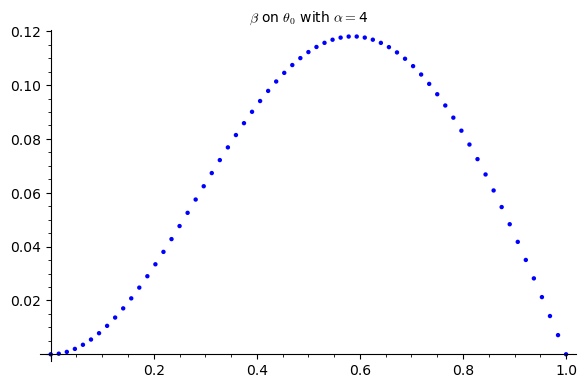
\includegraphics{output_39_1.png}
\caption{"$\beta on \theta_0 with \alpha = 4 $" }
\end{figure}
    
    Для грубо-оценочных расчётов положим $\beta = 0.1$

Зная разность концентраций молекул, способных по разные стороны от
мембраны проникнуть сквозь мембрану, можно грубо-ориентировочно,
воспользовавшись формулой для осмотического давления в разбавленных
растворах, оценить создаваемое на мембране немато-осмотическое давление:

\(p = \Delta c \cdot RT = \beta \cdot c \cdot RT\)

Это то давление, которое (подобно осмотическому) способна создать
мембрана при полной невозможности диффузионного потока.



    Плотность диффузионного потока:

\(J = -\,D \cdot \frac{dC}{dx}\)

плотность потока вещества \({\displaystyle J}\) (измеренная, например, в
\(моль \cdot м^{-2} с^{-1}\)) пропорциональна коэффициенту диффузии
\({\displaystyle D}\) {[}\(м^2·с^{-1}\){]} и градиенту концентрации. Это
уравнение выражает первый закон Фика.



    Осмотический поток растворителя через единицу площади мембраны
определяется по следующей формуле {[}2. Лазарев С.И., Коробов В.Б.,
Коновалов В.И. Исследование диффузионной и осмотической проницаемости
полимерных мембран. Тамбов. Тамб. Ин-т хим. машиностр, 1989. 12 с.{]}:

\(V_{ос} =\,\frac{Р_{ос}}{\delta}\left(С_{пер}-С_{рет}\right)\)

где \(V_{ос}\) --- осмотический поток растворителя, \(м/с\); \(\delta\)
--- толщина мембраны, \(м\); \(С_{пер}\), \(С_{рет}\) --- концентрации
пермеата и ретентата, соответственно; \(Р_{ос}\) --- коэффициент
осмотической проницаемости, \(м^5/\left(кг \cdot с\right)\).

Если в этом выражении концентрации выразить в молях на \(м^3\), то
коэффициент осмотической проницаемости получит размерность
\(м^5/\left(моль \cdot с\right)\), назовем такой коэффициент мольным
коэффициентом осмотической пронициемости.



    Диффузионный oсмотический поток в отсутствие давления, т.е. без
нагрузки, может быть найден как произведение разности концентраций
\(\Delta c = \beta \cdot c\) на отношение мольного коэффициента
осмотической проницаемости мембраны \(Р_{ос}\) к толщине мембраны. Далее
этот диффузионный oсмотический поток может быть выражен в единицах
объёма, делённых на единицу площади и времени, то есть в единицах
линейной скорости растворителя.

При его умножении на выше найденное немато-осмотическое давление и на
меньший единицы коэффициент \(\eta\) (коэффициент полезного действия, но
правильнее его называть коэффициентом неравновесности) может быть
выражена удельная мощность (мощность на единицу площади мембраны)
немато-осмотического двигателя.

\(w = \eta \cdot p \cdot V_{ос}\,\,\,\frac{Вт}{м^2}\)

    Диффузионный oсмотический поток:

\(V_{ос} = - \Delta c \cdot \frac{Р_{ос}}{\delta} = - \beta \cdot c \cdot \frac{Р_{ос}}{\delta} \frac{м}{с}\)

    Традиционный (или объёмный) коэффициент диффузии \(D\), встречающийся в
литературе, определяется, как отношение плотности диффузионного потока к
градиенту концентраций, поэтому он имеет размерность \(\frac{м^2}{с}\).

Если известен объёмный коэффициент диффузии для рабочего вещества в
мембране, то для оценки \(Р_{ос}\) --- мольного коэффициента
осмотической проницаемости, \(м^5/\left(моль \cdot с\right)\), мембраны,
можно объёмный коэффициент диффузии разделить на молярный объем,
\(моль/м^3\) (произведение молярной массы \(моль/кг\) и плотности
\(кг/м^3\)) и умножить на отношение площади пор к площади мембраны.

\(Р_{ос} = \frac{S_{пор}}{S_{мембр}}\cdot \frac{D}{\rho M}\)

    Формула для удельной мощности имеет вид:

\(w = \eta \cdot p \cdot V_{ос}\,\,\,\frac{Вт}{м^2}\)

\(w = \eta\cdot\beta\,c\,RT \cdot\beta\,c\frac{Р_{ос}}{\delta}\,\,\,\frac{Вт}{м^2}\)

    \(w = \eta\cdot\beta\,c\,RT \cdot\beta\,c\frac{\frac{S_{пор}}{S_{мембр}}\cdot \frac{D}{\rho\,M}}{\delta}\,\,\,\frac{Вт}{м^2}\)

\(w = \eta\cdot\beta^2\,c^2\,RT \cdot\frac{S_{пор}}{S_{мембр}}\cdot \frac{D}{\rho\,M\,\delta}\,\,\,\frac{Вт}{м^2}\)

    Для грубой оценки можно взять \(\eta=0.5\), \(c = 5\cdot10^3 моль/м^3\),
\(R=8.314\, Дж/моль\cdotК\), \(T = 300\,\), \(\beta=0.1\),
\(\delta = 10^-6\,м\)


eta=0.5
c = 5000
R = 8.314
T = 300
beta = 0.118037890843680
delta = 10e-6

%
%    \begin{tcolorbox}[breakable, size=fbox, boxrule=1pt, pad at break*=1mm,colback=cellbackground, colframe=cellborder]
%\prompt{In}{incolor}{54}{\boxspacing}
%\begin{Verbatim}[commandchars=\\\{\}]
%\PY{n}{eta}\PY{o}{=}\PY{l+m+mf}{0.5}
%\PY{n}{c} \PY{o}{=} \PY{l+m+mi}{5000}
%\PY{n}{R} \PY{o}{=} \PY{l+m+mf}{8.314}
%\PY{n}{T} \PY{o}{=} \PY{l+m+mi}{300}
%\PY{n}{beta} \PY{o}{=} \PY{l+m+mf}{0.118037890843680}
%\PY{n}{delta} \PY{o}{=} \PY{l+m+mi}{10}\PY{o}{\PYZca{}}\PY{o}{\PYZhy{}}\PY{l+m+mi}{6}
%\end{Verbatim}
%\end{tcolorbox}

% P_os = var("P_os")
$w =\ eta * \beta^2 * c^2 * R*T * P_{os}/(\delta)$
w

%    \begin{tcolorbox}[breakable, size=fbox, boxrule=1pt, pad at break*=1mm,colback=cellbackground, colframe=cellborder]
%\prompt{In}{incolor}{55}{\boxspacing}
%\begin{Verbatim}[commandchars=\\\{\}]
%\PY{n}{P\PYZus{}os} \PY{o}{=} \PY{n}{var}\PY{p}{(}\PY{l+s+s2}{\PYZdq{}}\PY{l+s+s2}{P\PYZus{}os}\PY{l+s+s2}{\PYZdq{}}\PY{p}{)}
%\PY{n}{w} \PY{o}{=} \PY{n}{eta} \PY{o}{*} \PY{n}{beta}\PY{o}{\PYZca{}}\PY{l+m+mi}{2} \PY{o}{*} \PY{n}{c}\PY{o}{\PYZca{}}\PY{l+m+mi}{2} \PY{o}{*} \PY{n}{R}\PY{o}{*}\PY{n}{T} \PY{o}{*} \PY{n}{P\PYZus{}os}\PY{o}{/}\PY{p}{(}\PY{n}{delta}\PY{p}{)}
%\PY{n}{w}
%\end{Verbatim}
%\end{tcolorbox}

%            \begin{tcolorbox}[breakable, size=fbox, boxrule=.5pt, pad at break*=1mm, opacityfill=0]
%\prompt{Out}{outcolor}{55}{\boxspacing}
%\begin{Verbatim}[commandchars=\\\{\}]
4.34394351421841e14*P\_os
%\end{Verbatim}
%\end{tcolorbox}
        
    Пусть \(\rho=10^3\,кг/м^3\), \(M = 0.2 \, кг/моль\),
\(\frac{S_{пор}}{S_{мембр}} = 0.1\), тогда

rho = 1000
M = 0.2
pore\_S\_part = 0.1

%    \begin{tcolorbox}[breakable, size=fbox, boxrule=1pt, pad at break*=1mm,colback=cellbackground, colframe=cellborder]
%\prompt{In}{incolor}{56}{\boxspacing}
%\begin{Verbatim}[commandchars=\\\{\}]
%\PY{n}{rho} \PY{o}{=} \PY{l+m+mi}{1000}
%\PY{n}{M} \PY{o}{=} \PY{l+m+mf}{0.2}
%\PY{n}{pore\PYZus{}S\PYZus{}part} \PY{o}{=} \PY{l+m+mf}{0.1}
%\end{Verbatim}
%\end{tcolorbox}

%D = var("D")
$P_{osm} = pore\_S\_part * D / (\rho * M)$
% P_osm

%    \begin{tcolorbox}[breakable, size=fbox, boxrule=1pt, pad at break*=1mm,colback=cellbackground, colframe=cellborder]
%\prompt{In}{incolor}{57}{\boxspacing}
%\begin{Verbatim}[commandchars=\\\{\}]
%\PY{n}{D} \PY{o}{=} \PY{n}{var}\PY{p}{(}\PY{l+s+s2}{\PYZdq{}}\PY{l+s+s2}{D}\PY{l+s+s2}{\PYZdq{}}\PY{p}{)}
%\PY{n}{P\PYZus{}osm} \PY{o}{=} \PY{n}{pore\PYZus{}S\PYZus{}part} \PY{o}{*} \PY{n}{D} \PY{o}{/} \PY{p}{(}\PY{n}{rho} \PY{o}{*} \PY{n}{M}\PY{p}{)}
%\PY{n}{P\PYZus{}osm}
%\end{Verbatim}
%\end{tcolorbox}

%            \begin{tcolorbox}[breakable, size=fbox, boxrule=.5pt, pad at break*=1mm, opacityfill=0]
%\prompt{Out}{outcolor}{57}{\boxspacing}
%\begin{Verbatim}[commandchars=\\\{\}]
0.000500000000000000*D
%\end{Verbatim}
%\end{tcolorbox}
        
    Из литературы {[}Импульсная спектроскопия ЯМР анизотропных материалов.
Автореферат диссертации, Двинских С.В. 2009{]} известен коэффициент
диффузии нематика в порах пористого стекла (диаметр пор 7 нм) в
приповерхностном слое \(D_{surf}=5\cdot10^{-14} м^2/с\), тогда как в
объёме нематика коэффициент диффузии \(D_{||}\approx10^{-10} м^2/с\) .


$D = 5*10e-14$
$P_{osm} = pore\_S\_part * D / (\rho * M)$
$P_{osm}$

%    \begin{tcolorbox}[breakable, size=fbox, boxrule=1pt, pad at break*=1mm,colback=cellbackground, colframe=cellborder]
%\prompt{In}{incolor}{58}{\boxspacing}
%\begin{Verbatim}[commandchars=\\\{\}]
%\PY{n}{D} \PY{o}{=} \PY{l+m+mi}{5}\PY{o}{*}\PY{l+m+mi}{10}\PY{o}{\PYZca{}}\PY{o}{\PYZhy{}}\PY{l+m+mi}{14}
%\PY{n}{P\PYZus{}osm} \PY{o}{=} \PY{n}{pore\PYZus{}S\PYZus{}part} \PY{o}{*} \PY{n}{D} \PY{o}{/} \PY{p}{(}\PY{n}{rho} \PY{o}{*} \PY{n}{M}\PY{p}{)}
%\PY{n}{P\PYZus{}osm}
%\end{Verbatim}
%\end{tcolorbox}

%            \begin{tcolorbox}[breakable, size=fbox, boxrule=.5pt, pad at break*=1mm, opacityfill=0]
%\prompt{Out}{outcolor}{58}{\boxspacing}
%\begin{Verbatim}[commandchars=\\\{\}]
2.50000000000000e-17
%\end{Verbatim}
%\end{tcolorbox}

$w = \eta * \beta^2 * c^2 * R*T * pore\_S\_part * D / (\rho * M * \delta)$
w
        
%    \begin{tcolorbox}[breakable, size=fbox, boxrule=1pt, pad at break*=1mm,colback=cellbackground, colframe=cellborder]
%\prompt{In}{incolor}{59}{\boxspacing}
%\begin{Verbatim}[commandchars=\\\{\}]
%\PY{n}{w} \PY{o}{=} \PY{n}{eta} \PY{o}{*} \PY{n}{beta}\PY{o}{\PYZca{}}\PY{l+m+mi}{2} \PY{o}{*} \PY{n}{c}\PY{o}{\PYZca{}}\PY{l+m+mi}{2} \PY{o}{*} \PY{n}{R}\PY{o}{*}\PY{n}{T} \PY{o}{*} \PY{n}{pore\PYZus{}S\PYZus{}part} \PY{o}{*} \PY{n}{D} \PY{o}{/} \PY{p}{(}\PY{n}{rho} \PY{o}{*} \PY{n}{M} \PY{o}{*} \PY{n}{delta}\PY{p}{)}
%\PY{n}{w}
%\end{Verbatim}
%\end{tcolorbox}
%
%            \begin{tcolorbox}[breakable, size=fbox, boxrule=.5pt, pad at break*=1mm, opacityfill=0]
%\prompt{Out}{outcolor}{59}{\boxspacing}
%\begin{Verbatim}[commandchars=\\\{\}]
0.0108598587855460
%\end{Verbatim}
%\end{tcolorbox}
        
    итак, \(w \approx 10.86\,мВт/м^2\). Если взять мембрану толщиной 1
микрон и площадью 10 на 10 сантиметров, то мощность снимаемая с одной
такой мембраны будет порядка \(0.1086\,мВт\). Но если сделать стопку
таких мембран общей высотой 10 сантиметров, то при расстоянии между
мембранами 9 микрон можно иметь в такой стопке 100 тысяч мембран. Тогда
суммарная мощность такой мембранной системы может достигать
\(10.85\,Ватт\).

$w*10^{5}/100$

%    \begin{tcolorbox}[breakable, size=fbox, boxrule=1pt, pad at break*=1mm,colback=cellbackground, colframe=cellborder]
%\prompt{In}{incolor}{60}{\boxspacing}
%\begin{Verbatim}[commandchars=\\\{\}]
%\PY{n}{w}\PY{o}{*}\PY{l+m+mi}{10}\PY{o}{\PYZca{}}\PY{l+m+mi}{5}\PY{o}{/}\PY{l+m+mi}{100}
%\end{Verbatim}
%\end{tcolorbox}

%            \begin{tcolorbox}[breakable, size=fbox, boxrule=.5pt, pad at break*=1mm, opacityfill=0]
%\prompt{Out}{outcolor}{60}{\boxspacing}
%\begin{Verbatim}[commandchars=\\\{\}]
10.8598587855460
%\end{Verbatim}
%\end{tcolorbox}
        
    Если удастся уменьшить в 10 раз толщину мембраны (доведя толщину
мембраны до одной десятой микрона) можно таким образом и ожидаемую
мощность кубического дециметра мембранного пакета довести до
\(108.5\,Ватт\).

Лимитирующими факторами здесь являются минимальная технологически
достижимая толщина трековой мембраны и максимально допустимая плотность
упаковки мембран, определяемая по сути упругими свойствами нематика: это
та толшина слоя нематика в которой он может легко без дисклинаций
поменять в своей толще планарную ориентацию на гомеотропную.

    Анализ функций распределения ориентации молекул по разные стороны от
мембраны (т.е. разницы двух функций распределения, одина из которых
смещёна на \(\pi/2\) ) позволяет заключить, что достигнуть максимального
значения коэффициента \(\beta\) (равного 0.118037890843680) возможно при
\(\theta_0 = 19/64 \pi\).

Отсюда мы можем заключить, что наиболее оптимальное значение
эффективного диаметра капилляра равно:

\(d_{эф} = длина\_молекулы\_нематика \cdot sin\, \theta_0\)

Например, длина молекулы 5ЦБ \(\approx 1.2\,нм\), откуда требуемый
эффективный диаметр пор \(d_{эф} = 0.96\,нм\).


1.2*sin(19/64*pi).n()

%    \begin{tcolorbox}[breakable, size=fbox, boxrule=1pt, pad at break*=1mm,colback=cellbackground, colframe=cellborder]
%\prompt{In}{incolor}{61}{\boxspacing}
%\begin{Verbatim}[commandchars=\\\{\}]
%\PY{l+m+mf}{1.2}\PY{o}{*}\PY{n}{sin}\PY{p}{(}\PY{l+m+mi}{19}\PY{o}{/}\PY{l+m+mi}{64}\PY{o}{*}\PY{n}{pi}\PY{p}{)}\PY{o}{.}\PY{n}{n}\PY{p}{(}\PY{p}{)}
%\end{Verbatim}
%\end{tcolorbox}

%            \begin{tcolorbox}[breakable, size=fbox, boxrule=.5pt, pad at break*=1mm, opacityfill=0]
%\prompt{Out}{outcolor}{61}{\boxspacing}
%\begin{Verbatim}[commandchars=\\\{\}]
0.963849037776774
%\end{Verbatim}
%\end{tcolorbox}
        
    \section{Дискуссия}\label{ux434ux438ux441ux43aux443ux441ux441ux438ux44f}

    Возвращаясь к обсуждавшемуся в начале обоснованию принципа детального
равновесия следует отметить следующее. В классической механике,
действительно, все состояния разрешены. В том смысле, что в классической
механике нет таких запретов на состояния, которые существуют в квантовой
механике (т.е. запретов основанных на свойствах волновой функции). Но с
другой стороны, классические системы могут содержать
пространственно-стерические или кинетические в результате чего два
состояния, отличающиеся лишь направлением скоростей молекул, имеющие
вследствие симметрии пространства одинаковые кинетические и
потенциальные энергии, могут иметь всё же различные вероятности
реализации. Таким образом, left-right несимметричные пространственные
затруднения в классических молекулярных системах могут приводить к
отклонениям от принципа детального равновесия.

Является ли предполагаемая в данной работе модель жидкокристаллического
осмоса разновидностью фейнмановского храповика и собачки? В некотором
смысле да. В своей известной лекции Фейнман, доказывая
неработоспособность своей системы, указывал на хаотические (т.е. на
нескоррелированные) броуновские колебания как храповика так и собачки,
однако существуют как минимум две возможности возразить против данной
аргументации Фейнмана:

\begin{enumerate}
\def\labelenumi{\arabic{enumi})}
\item
  возможность храповиков и собачек совместно участвовать в
  длинноволновых (с длиной волны большей храпового шага) фононных
  колебаниях. Что вносит в броуновское движение храповиков и собачек
  коллективную составляющую и соответственно приводит к корреляции.
  Такая возможность может реализовываться в системе наклонённых под
  углом 45 градусов молекул ориентантов, выступающих в роли, скажем,
  собачек, и системе аналогично ориентированных молекул жидкого
  кристалла (храповиков). Эта идея была предложена в работе
  {[}«Жидкокристаллический двигатель»{]}.
\item
  В данной работе {[}«Жидкокристаллический осмос»{]} в роли храповиков
  выступают молекулы жидких кристаллов, а в роли собачек -- поры или
  капилляры. Однако здесь есть две особенности:
\end{enumerate}

а) храповики и собачки находятся в разных фазах, - храповики в жидкой,
собачки в твёрдой. Поэтому колебания собачек в результате теплового
движения имеет намного меньшую амплитуду, чем колебания храповиков. Это
приводит к тому, что изменением диаметра пор в результате теплового
движения можно пренебречь по сравнением с изменением вертикальной
проекции сечения молекул нематика в результате изменения их ориентации.
Эта особенность полностью сводит на нет довод Фейнмана о хаотичности
броуновского движения храповика и собачки.

б) вторая особенность состоит в том, что собственно храповые свойства
возникают благодаря ориентирующим свойствам всей массы жидкого кристалла
и различным граничным условиям по разные стороны от мембраны.

    \section{О механизме
осмоса}\label{ux43e-ux43cux435ux445ux430ux43dux438ux437ux43cux435-ux43eux441ux43cux43eux441ux430}

    Что есть механизмом осмоса?

\begin{itemize}
\item
  Вот например цитата из википедии: "осмотическое давление возникает
  соответственно Принципу Ле Шателье из-за того, что система пытается
  выровнять концентрацию раствора в обеих средах, разделённых мембраной,
  и описывается вторым законом термодинамики. " То есть общепринятый
  механизм осмоса ничего не говорит об асимметричной на молекулярном
  уровне проницаемости мембран.
\item
  Моё видение причин осмоса основано на том, что вероятность
  проникновения молекулы растворителя в (симметричную) мембрану зависит
  от концентрации растворенного вещества. И именно разница вероятностей
  создает давление. Исходя именно из такого видения я предположил
  возможность создания осмотического давления также и без растворенного
  вещества но при разных граничных условиях для нематика для в общем-то
  симметричной (с цилиндрическими порами, хотя и с различной по
  обработке поверхностями) мембраной.
\end{itemize}

Нужно терминологически различать "механизм осмоса" официальный (Ле
Шателье и второе начало) от механизма осмоса вероятностного с
предполагаемым нарушением принципа детального равновесия на
асимметричных мембранах.

    \section{Границы применимости второго начала
термодинамики}\label{ux433ux440ux430ux43dux438ux446ux44b-ux43fux440ux438ux43cux435ux43dux438ux43cux43eux441ux442ux438-ux432ux442ux43eux440ux43eux433ux43e-ux43dux430ux447ux430ux43bux430-ux442ux435ux440ux43cux43eux434ux438ux43dux430ux43cux438ux43aux438}

    Цитата из википедии:

В системе идей Клаузиуса и его последователей оба принципа существования
и возрастания энтропии основываются на постулате необратимости
(постулаты Клаузиуса, Томсона-Кельвина, Планка и др.), причём во главу
угла поставлен принцип возрастания энтропии, который возводится в ранг
универсального закона природы, стоящего рядом с законом сохранения
энергии. Абсолютизация Клаузиусом принципа возрастания энтропии
приобрела смысл важнейшего космологического закона природы, следствием
которого стала антинаучная концепция «тепловой смерти Вселенной».
{[}44{]} Таким образом, любое нарушение этого фундаментального закона
привело бы к обрушению всех следствий из него, что существенно
ограничило бы сферу влияния термодинамики. Характерным в этом смысле
является высказывание М. Планка, утверждавшего, что с необратимостью
«стоит и падает термодинамика». В этом смысле выводы статистической
физики о вероятностном характере принципа необратимости и открытие
систем с отрицательными абсолютными температурами должны привести к
краху второго начала, а вместе с ним и самой термодинамики. Однако это
не произошло. Ошибочный вывод М. Планка о «падении термодинамики» с
падением постулата необратимости непосредственно связан с сложившимся
исторически, объединении в одном законе принципов существования и
возрастания энтропии и придание принципу возрастания энтропии смысла
второго начала термодинамики. На неравноценность указанных принципов и
несовместимость их в одном начале термодинамики обратила внимание Т.
Афанасьева-Эренфест. По её словам, одно и то же начало представляется в
двух совершенно различных обликах: 1) как утверждение существования
интегрирующего множителя для известного выражения dQ и 2) как
утверждение о неуклонном возрастании энтропии при реальных
адиабатических процессах. Представляется трудным уместить в одно
отчетливое обозримое поле зрения эти оба положения и схватить логическое
тождество второго начала и принципа возрастания энтропии.{[}45{]}

Благодаря ревизии второго начала термодинамики на первый план в качестве
фундаментального закона термодинамики выходит принцип существования
энтропии, а принцип возрастания энтропии изолированных систем является
принципом локальным, статистическим, который, по словам
Афанасьевой-Эренфест, выполняется «только в некоторые эпохи».{[}46{]}

Немного перефразирую: принцип возрастания энтропии изолированных систем
является принципом вероятностным

Это к вопросу о том, что рассматривая механизм осмоса именно как
вероятностный процесс можно на асимметричных мембранах добиться того,
что снижения энтропии окажется более вероятным чем ее возрастание




    % Add a bibliography block to the postdoc
    
    
    
\end{document}
